\documentclass{article}
\usepackage{package}
\graphicspath{ {./images/} }

\title{
    {\LARGE Relazione del Progetto di Programmazione Web e Mobile}\\
    (PWM)\\
    %\vskip 0.8 cm{\Large Facolt\`a di Scienze e Tecnologie}\\
    \vskip 0.4cm{\large Dipartimento di Informatica Giovanni Degli Antoni}
}
\author{
    \Large Samuele Manclossi\\
    \large 09882A
}
\date{
    {\large\today}
}


\begin{document}
\pagenumbering{gobble}

\begin{titlepage}
    \pagestyle{empty}
    \selectlanguage{italian}
    \maketitle
    \selectlanguage{italian}
    \vspace{1em}
    \epigraph{\say{Non quia difficilia sunt non audemos, sed quia non audemos difficilia sunt}}{--- \textup{Seneca}}
    \selectlanguage{english}
    \vspace{2em}
    \begin{abstract}
        \textit{Questo PDF è la relazione del progetto conclusivo del corso di Programmazione Web e Mobile, tenuto dal prof. Valerio Bellandi alla Università Statale di Milano nell'A.A. 2022-2023.

Esso consiste nella realizzazione di una applicazoine web dal nome \uppercase{Social Network for Music}, che si deve prefiggere lo scopo principale di implementare un sistema di gestione delle playlist musicali create da utenti ed (eventualmente) condivise.}
        %\textit{\kant[1]}% TODO 
    \end{abstract}
    \vskip 4cm\centerline{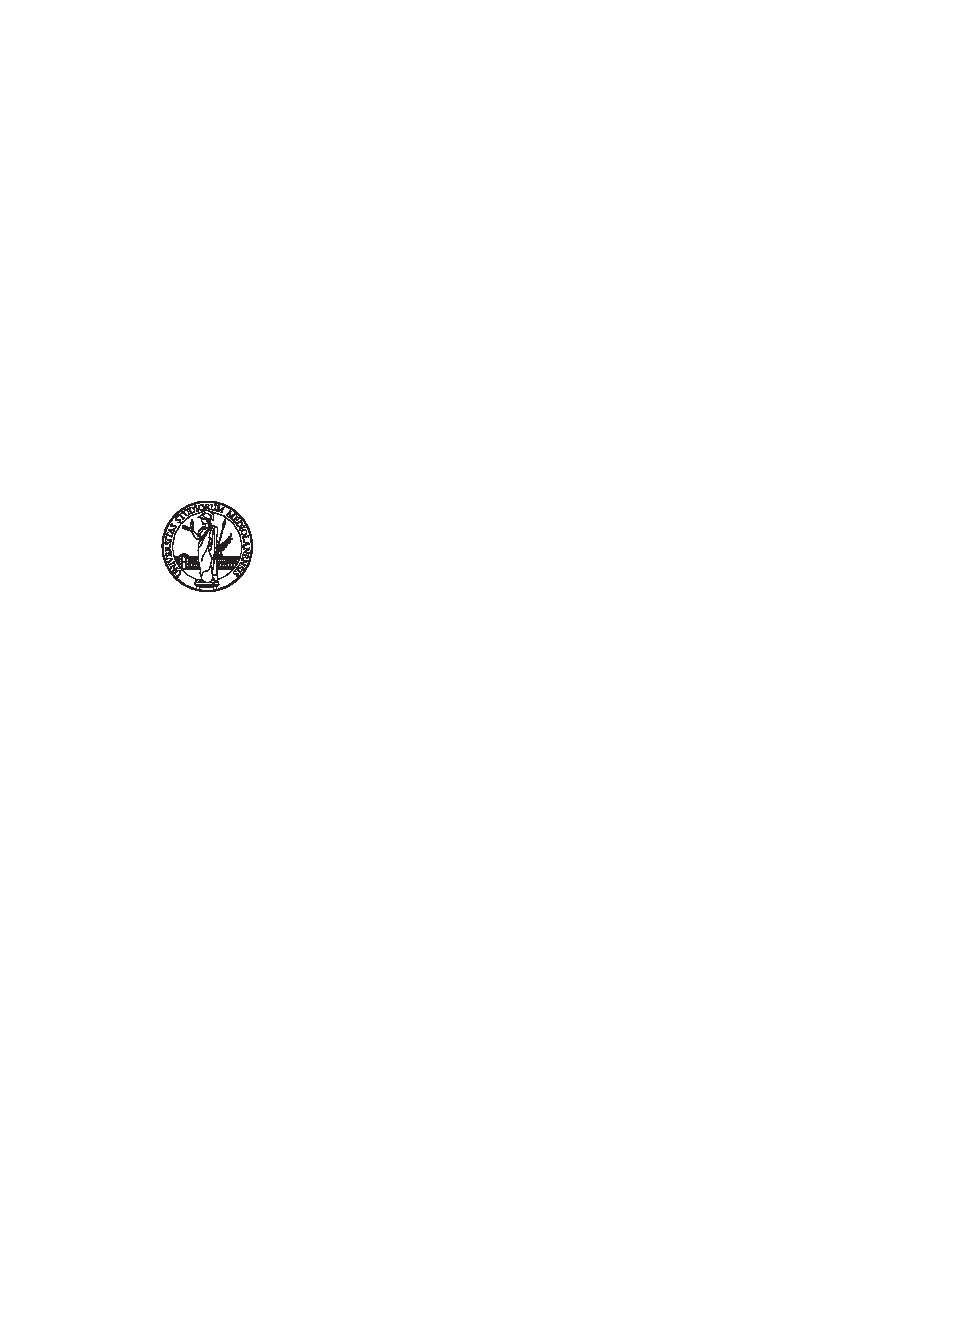
\includegraphics[height=50mm]{./src/unimi}}
    \newpage
    \pagenumbering{Roman}
    \tableofcontents
    \selectlanguage{italian}
    \vspace{\fill}
\end{titlepage}

\pagenumbering{arabic}
\lhead{Programmazione Web e Mobile}
\rhead{Samuele Manclossi}

\selectlanguage{italian}
\section{Analisi delle specifiche}
\subsection{Funzionalità da implementare}
\uppercase{Social Network for Music} (di seguito \verb|SNM|) deve essere in grado di svolgere diverse funzioni, tra cui le seguenti.

Si noti, non saranno riportati i campi dei singoli oggetti, in quanto essi sono già presenti nella apposita sezione riguardante la struttura dati, all'interno delle scelte implementative.
\subsubsection{Gestione degli utenti}
La gestione degli utenti è necessaria, e deve essere affrontata attraverso diverse fasi:
\paragraph{Registrazione} La registrazione degli utenti avviene attraverso una pagina apposita, a cui può accedere qualsiasi utente. Questa pagina consente (dopo appositi controlli) di effettuare una richiesta POST al backend, che si occuperà di registrare i dati dopo averli nuovamente verificati.

I campi che saranno richiesti in fase di registrazione dovranno essere:
\begin{itemize}
    \item \textbf{Email}, campo unico che verrà usato per autenticarsi.
    \item \textbf{Password}
    \item \textbf{Conferma password}
    \item \textbf{Nome utente}, che sarà il nome mostrato agli altri quando una playlist viene condivisa e per simili funzionalità
    \item \textbf{Preferenze musicali} (genere preferito, da una lista restituita dal backend)
    \item \textbf{Gruppi musicali preferiti}
\end{itemize}
\idea{Per ragioni implementative, i gruppi musicali preferiti di default saranno vuoti, come ogni altro preferito. Questi potranno essere infatti aggiunti in maniera più corretta e coerente con il resto dell'applicazione navigando e cercando i gruppi, in modo da salvarne gli ID coerentemente con quelli forniti da Spotify}
\paragraph{Login} Mediante il login un utente entra nel proprio profilo, diventando in grado di vedere le proprie playlist e il proprio profilo.

Questo avverrà attraverso la richiesta di due campi:
\begin{itemize}
    \item Email
    \item Password
\end{itemize}
Entrambi i campi saranno modificabili da un apposito sistema.

Nonostante sia stato suggerito di salvarsi le informazioni in locale sarebbe più opportuno usare i token JWT. A questo sarà dedicata una apposita sezione.
\paragraph{Logout} Questa funzione si spiega da sola, senza bisogno di tanti commenti.
\paragraph{Cambiare i propri dati} Ogni dato deve essere modificabile tramite apposite richieste al backend.
\paragraph{Eliminare l'account} Deve essere possibile eliminare l'account, cancellando tutte le informazioni che lo riguardano. Se l'account viene eliminato, vengono rimosse tutte le playlist create da quell'utente. Sarebbe pertanto consigliabile la realizzazione di un sistema che consenta, all'eliminazione dell'account, di stabilire a chi passa la proprietà di quelle playlist, oppure scegliere di eliminarle.
\subsubsection{Ricerca e visualizzazione dei dati}
Questo deve essere fatto attraverso due pagine apposite, una che si occupi della ricerca e ne mostri i risultati e una che mostri le informazioni sul singolo brano, permettendo l'inserimento di questo nelle playlist (eventualmente la creazione di una nuova playlist in caso non dovesse già esistere).

Vista l'ampia varietà di campi per cui è possibile cercare, una soluzione sarebbe prima mostrare alcuni risultati per ogni campo e poi restringere la ricerca su un campo specifico.
\subsubsection{Preferiti e Playlist}
\paragraph{Preferiti} Un utente può decidere di selezionare un numero imprecisato di brani come suoi brani preferiti. Questo li aggiunge alle informazioni (private) del suo account. Non solo, egli potrà inserire potenzialmente ogni categoria di dati restituiti da Spotify.
\paragraph{Playlist} Una playlist è una collezione di brani denotata da alcune informazioni, ritrovabili nella sezione apposita.

Una playlist privata può essere vista solamente dal creatore, una playlist pubblica può essere vista liberamente da chiunque mediante una apposita pagina, mentre una playlist condivisa con un gruppo può essere visibile a chiunque sia all'interno di quella 

Si noti che le playlist devono implementare le seguenti azioni:\begin{itemize}
    \item \textbf{Cancellazione}
    \item \textbf{Rendere privata}
    \item \textbf{Rendere pubblica}
    \item \textbf{Condividere con un gruppo}
    \item \textbf{Rimuovere condivisione con un gruppo}
    \item \textbf{Follow/Unfollow}
    \item \textbf{Trasferimento della proprietà ad un nuovo owner}
    \item \textbf{Aggiunta o Rimozione di canzoni}
    \item \textbf{Recuperare le informazioni}
\end{itemize}
\subsubsection{Opzionale: creazione di gruppi}
Si potranno creare delle comunità di utenti, di qui in avanti \verb|gruppi|, a cui gli utenti potranno iscriversi e disiscriversi. Quando un utente è iscritto, esso è in grado di vedere tutte le playlist condivise con quella comunità specifica, e risulta anche in grado di parteciparvi condividendo altre playlist.

Il creatore del gruppo non può essere in grado di escludere qualcuno dal gruppo. Questo perché i gruppi nascono come comunità aperte. Il creatore del gruppo, però, ipoteticamente, potrebbe essere in grado di annullare le condivisioni di playlist verso quel gruppo da parte di altri, cosa che agli utenti normali non è consentita.

\alert{Nel momento in cui esco da un gruppo, ogni playlist che avevo condiviso con quel gruppo viene rimossa dal gruppo. Se invece stavo seguendo una playlist, quella playlist rimane seguita, anche se non potrò più accedervi se non rientrando nel gruppo.}

\alert{Quando trasferisco la proprietà di una playlist a qualcuno non nel gruppo con cui è condivisa, questa rimane condivisa. Non consiste in una perdita di integrità, ma piuttosto nel rispettare la volontà di chi l'ha trasferita senza prima toglierla dal gruppo.}
\newpage
\section{Tecnologie utilizzate e interazioni tra esse}
Le tecnologie utilizzate saranno divise a seconda della tipologia.
\subsection{Data}
Per i dati si è utilizzato, come da istruzioni ricevute, MongoDB. La struttura dati è approfondita nelle scelte progettuali, come anche l'uso delle informazioni di accesso, pertanto non vi sono altre informazioni rilevanti da specificare in questa sede.
\subsection{Backend}
Per il backend si è utilizzato \href{https://nodejs.org/en/about}{NodeJS}, con l'utilizzo del framework \verb|express|\cite{express}.

L'utilizzo di \verb|NPM| ha consentito l'uso dei package, in particolare sono stati usati:
\begin{itemize}
    \item \textbf{cookie-parser}: un package che consente di parsare l'header \verb|Cookie| e popolare \verb|req.cookies| con un oggetto avente per attributi i nomi dei cookie\cite{cookie-parser}.
    \item \textbf{cors}: un middleware per eliminare i fastidiosi problemi con i cors\cite{cors}.
    \item \textbf{dotenv}: un package per la gestione del \verb|.env|, con un comodo comando \verb|require('path/to/file')| e di seguito \verb|.configure()|\cite{dotenv}.
    \item \textbf{express}: il framework già citato sopra.
    \item \textbf{express-mongo-sanitize}: un package che fornisce un middleware per la sanitizzazione di molti campi delle richieste. Si noti che l'ho usato con la configurazione \verb|allowDots: true| per evitare che l'email venisse modificata. Per il resto consente un notevole miglioramento della sicurezza con riduzione del rischio di injections\cite{express-mongo-sanitize}.
    \item \textbf{jsonwebtoken}: il package che consente una autenticazione un po' più sicura rispetto al minimo richiesto mediante l'uso, la firma e la verifica dei \verb|JWT| tramite comodi metodi\cite{jsonwebtoken}.
    \item \textbf{mongodb}: il package ufficiale per gestire MongoDB da NodeJS\cite{mongodb-npm}
    \item \textbf{nodemon}: un package che consente di riavviare il server nel momento in cui rileva qualsiasi cambiamento\cite{nodemon}.
    \item \textbf{swagger-ui-express}: un package per fornire uno swagger\cite{swagger-ui-express}
    \item \textbf{validator}: un package molto utile per sanitizzare e validare stringhe\cite{validator}.
    \item[*] \textbf{swagger-autogen}: utilizzato solo come \verb|devDependency|, esso è utile per generare automaticamente lo swagger\cite{swagger-autogen}. L'export di questo swagger lo trovate nell'Appendice C.
\end{itemize}
Ci sono poi altri packages, come \verb|crypto| o \verb|path|, che venivano già forniti in automatico.

Il file \verb|package.json| risulta quindi composto come segue:
\begin{lstlisting}[language=JavaScript]
{
    "scripts": {
        "start": "nodemon app.js",
        "debug": "nodemon --inspect app.js"
    },
    "dependencies": {
        "cookie-parser": "^1.4.6",
        "cors": "^2.8.5",
        "dotenv": "^16.0.3",
        "express": "^4.18.2",
        "express-mongo-sanitize": "^2.2.0",
        "jsonwebtoken": "^9.0.0",
        "mongodb": "^5.4.0",
        "nodemon": "^1.14.9",
        "swagger-ui-express": "^4.6.2",
        "validator": "^13.9.0"
    },
    "devDependencies": {
        "swagger-autogen": "^2.23.1"
    }
}
\end{lstlisting}
\subsection{Frontend}
Le tecnologie usate lato frontend sono HTML5, CSS3 e JavaScript, con l'utilizzo di \href{https://getbootstrap.com/}{\underline{Bootstrap 5.3}}. Per le scelte implementative si faccia riferimento all'apposita sezione.

Unica tecnologia significativa usata è stata una libreria: in classe era stato suggerito di poter modificare l'ordine delle canzoni in una playlist. Per farlo, ho usato una libreria per facilitare il drag and drop delle cards. Questa libreria è \href{https://sortablejs.github.io/Sortable/}{\underline{SortableJS}}, che consente giusto di ottenere l'effetto di riposizionamento.

Non è stato usato altro codice esterno.
\newpage
\section{Interfaccia utente e front-end}
\subsection{Pagine e relative funzioni e visibilità}
\subsubsection{Pagine non richiedenti login}
\paragraph{Welcome page - \textit{index.html}}
La pagina di accoglienza sarà una pagina con pochissime funzionalità, destinata prevalentemente a fare da \say{vetrina} del servizio offerto. Da essa si potranno trovare i link a tutte le altre funzionalità.

Vi saranno due pulsanti: \verb|login| e \verb|register|, e la navbar per navigare invece la parte pubblica.

\paragraph{Registrazione - \textit{register.html}}
La pagina di registrazione sarà costituita da un form. Se si è loggati, si verrà reindirizzati automaticamente alla pagina di login. Altrimenti, ci si potrà registrare. Se la registrazione va a buon fine si viene reindirizzati alla pagina di login, altrimenti viene mostrato il messaggio d'errore restituito dal backend.

\paragraph{Login - \textit{login.html}}
La pagina di login sarà costituita da un form. Se si è già loggati si viene reindirizzati alla pagina richiesta mediante un parametro, altrimenti ci si può loggare. In ogni caso saranno emessi appositi messaggi per segnalare lo stato.

\paragraph{Ricerca - \textit{search.html}}
La pagina di ricerca consentirà di effettuare una ricerca per vari campi. Una volta cercato, verranno mostrati i primi risultati di ogni categoria. Se si desidera ottenere maggiori risultati di quella categoria, i parametri vengono ristretti mentre avviene la redirezione a una pagina apposita.
\alert{Al momento non è possibile filtrare i risultati: ho preferito dare la possibilità di selezionare più categorie piuttosto che limitare i risultati. Questo potrebbe diventare uno sviluppo futuro}
\paragraph{Not Found - \textit{not\_found.html}}
Questa pagina sarà quella mostrata ogniqualvolta sia stata richiesta una pagina non esistente.

\subsubsection{Pagine richiedenti login}
\paragraph{Playlist - \textit{playlists.html}}
In questa pagina si potranno cercare le playlist pubbliche o comunque condivise con sé, e crearne di nuove.

\paragraph{Groups - \textit{groups.html}}
Questa pagina consentirà la creazione, la visualizzazione e il filtraggio dei gruppi.

\paragraph{Spiegazione di una playlist o di un gruppo \textit{explainPlaylist.html|explainGroup.html}}
Come la pagina di \verb|describe|, ma per playlist o gruppi. Dovranno includere l'unirsi e l'uscire dai gruppi, l'unire o il rimuovere una playlist a un gruppo e una canzone ad una playlist.
\paragraph{Profilo - \textit{profile.html}}
Questa pagina includerà tutte le informazioni legate all'utente, come preferiti, dati personali, playlist seguite o possedute, gruppi in cui si è o posseduti.


\subsection{Navbar condivisa tra tutte le pagine}
Tutte le pagine avranno accesso a una navbar condivisa, costituita dai seguenti elementi.
\subsubsection{Pulsante \textit{SNM}}
Permette di tornare alla pagina \verb|index.html|.
\subsubsection{Pulsante \textit{Playlists}}
Consente di tornare alla pagina delle playlist pubbliche.
\subsubsection{Pulsante \textit{Search}}
Consente di tornare alla pagina di ricerca.
\subsubsection{Pulsante \textit{Groups}}
Consente di tornare alla pagina dove sono mostrati i gruppi, ed eventualmente visualizzare le informazioni su di essi.
\subsubsection{Dropdown \textit{User}}
Esso conterrà diverse operazioni sul profilo, tra cui le seguenti:
\paragraph{Register}Visibile solo a chi non è loggato, permette di registrarsi.
\paragraph{Login}Visibile solo a chi non è loggato, permette di loggarsi.
\paragraph{Logout}Visibile solo a chi è loggato, permette di effettuare il logout.
\paragraph{My Favorites}Visibile solo a chi è loggato, permette di andare al profilo, nella sezione dedicata ai preferiti.
\paragraph{My Playlists}Visibile solo a chi è loggato, permette di andare al profilo, nella sezione dedicata alle playlists.
\paragraph{My Groups}Visibile solo a chi è loggato, permette di andare al profilo, nella sezione dedicata ai gruppi.
\paragraph{Profile}Visibile solo a chi è loggato, permette di andare al profilo.
\newpage
\section{Appendice A: brani di codice}
\section{Appendice B: response status}
\end{document}